
%-------------------------------------------------------------------------------
%                             ADDITIONAL PACKAGES
%-------------------------------------------------------------------------------
\documentclass[
	a4paper,
%	showframes,
%	vline=2.2em,
%	maincolor=cvgreen,
%	sectioncolor=red,
%	subsectioncolor=orange,
%	itemtextcolor=black!80,
%	sidebarwidth=0.4\paperwidth,
%	topbottommargin=0.03\paperheight,
%	leftrightmargin=20pt,
%	profilepicsize=4.5cm,
%	profilepicborderwidth=3.5pt,
%	profilepicstyle=profilecircle,
%	profilepiczoom=1.0,
%	profilepicxshift=0mm,
%	profilepicyshift=0mm,
% profilepicrounding=1.0cm,
]{fortysecondscv}

% define divider and cvdivider command: dashed gray line separator
% attention: import colortbl befor arydshln
\usepackage{colortbl}
\usepackage{arydshln}
\RequirePackage{dashrule}
\colorlet{body}{black!80!white}
\newcommand{\cvdivider}{\arrayrulecolor{body!30}\hdashline}
\newcommand{\profiledivider}{\textcolor{body!30}{\hdashrule{\linewidth}{0.6pt}{0.5ex}}\\}
%\newcommand{\divider}{\textcolor{body!30}{\hdashrule{\linewidth}{0.6pt}{0.5ex}}}

% Portuguese package (used in signature date)
%\usepackage[portuguese]{babel}

% package used to wrap text around a figure
\usepackage{wrapfig}

% provides blind text useful for test purposes
\usepackage{blindtext}

\usepackage{amsmath}
\usepackage{makecell}

% table related packages
\usepackage{multirow}
\usepackage{array}
\newcolumntype{L}[1]{>{\raggedright\let\newline\\\arraybackslash\hspace{0pt}}m{#1}}
\newcolumntype{C}[1]{>{\centering\let\newline\\\arraybackslash\hspace{0pt}}m{#1}}
\newcolumntype{R}[1]{>{\raggedleft\let\newline\\\arraybackslash\hspace{0pt}}m{#1}}

% floating objects (figures, tables)
\usepackage{float}
% set font to any desired size
%\usepackage{anyfontsize}
% add font sizes \HUGE and \ssmall
%\usepackage[11pt]{moresize}

% multiple columns
\usepackage{multicol}
\usepackage{vwcol}

% adjust list spacing
\usepackage{enumitem}

% include fonts
\pdfmapfile{=ClearSans.map}
\pdfmapfile{=fontawesome.map}

% include and use scalable cm-super fonts
\usepackage[T1]{fontenc}
\usepackage{lmodern}

% improve word spacing and hyphenation
\usepackage{microtype}
\usepackage{ragged2e}

% provides blind text useful for test purposes
\usepackage{blindtext}

\usepackage{amsmath}

% include fonts
\pdfmapfile{=ClearSans.map}
\pdfmapfile{=fontawesome.map}

% include and use scalable cm-super fonts
\usepackage[T1]{fontenc}
\usepackage{lmodern}

% improve word spacing and hyphenation
\usepackage{microtype}
\usepackage{ragged2e}

% take care of proper font encoding
\ifxetexorluatex
	\usepackage{fontspec}
	\defaultfontfeatures{Ligatures=TeX}
%	\newfontfamily\headingfont[Path = fonts/]{segoeuib.ttf} % local font
\else
	\usepackage[utf8]{inputenc}
	\usepackage[T1]{fontenc}
%	\usepackage[sfdefault]{noto} % use noto google font
\fi

% enable mathematical syntax for some symbols like \varnothing
\usepackage{amssymb}

% bubble diagram configuration
%\usepackage{smartdiagram}
%\smartdiagramset{
%	% default font size is \large, so adjust to harmonize with sidebar layout
%	bubble center node font = \footnotesize,
%	bubble node font = \footnotesize,
%	% default: 4cm/2.5cm; make minimum diameter relative to sidebar size
%	bubble center node size = 0.4\sidebartextwidth,
%	bubble node size = 0.25\sidebartextwidth,
%	distance center/other bubbles = 1.5em,
%	% set center bubble color
%	bubble center node color = maincolor!70,
%	% define the list of colors usable in the diagram
%	set color list = {maincolor!10, maincolor!40,
%	maincolor!20, maincolor!60, maincolor!35},
%	% sets the opacity at which the bubbles are shown
%	bubble fill opacity = 0.8,
%}


%-------------------------------------------------------------------------------
%                            PERSONAL INFORMATION
%-------------------------------------------------------------------------------
%% mandatory information
% your name
\cvname{Rafael Claro Ito}
% job title/career
\cvjobtitle{
    Electrical Engineer\\[0.2em]
    HW \& SW Developer\\[0.2em]
    Data Scientist
}






%\graphicspath{{../figures/whoami/}}
%\newcommand{\whoamiemail}{\cvicon{\includegraphics[align=c, width=1.0em]{email}}}
%\whoamiemail




%% optional information
% profile picture
\cvprofilepic{../figures/profile.jpeg}

% NOTE: ordering in sidebar will mimic the following order
% date of birth
\cvbirthday{03/02/1992}
% short address/location, use \newline if more than 1 line is required
%\cvaddressone{Rua Gilberto Pattaro, 150 $\cdot$ Campinas/SP, Brazil}
\cvaddressone{Rua Gilberto Pattaro, 150 $\boldsymbol{\cdot}$ 13084-375}
\cvaddresstwo{Campinas, SP $\boldsymbol{\cdot}$ Brazil}
% phone number
\cvphone{+55 19 98810-2615}
% personal website
%\cvsite{https://pandascience.net}
% email address
\cvmail{ito.rafael@gmail.com}
% pgp key
%\cvkey{4096R/FF00FF00}{0xAABBCCDDFF00FF00}
% any other custom entry
%\cvcustomdata{\faFlag}{Chinese}

%\cvline{\hline}
%\cvline{}

\cvlinkedin{https://www.linkedin.com/in/itorafael/}{linkedin.com/in/itorafael}
\cvgithub{https://github.com/ito-rafael/}{github.com/ito-rafael}
\cvfacebook{https://www.facebook.com/ito.rafael92}{facebook.com/ito.rafael92}
\cvskype{}{ito.rafael92}

%-------------------------------------------------------------------------------
%                              SIDEBAR 1st PAGE
%-------------------------------------------------------------------------------
% add more profile sections to sidebar on first page
\addtofrontsidebar{

%    %===============
%    % SOCIAL NETWORK
%    %===============
%	% social network accounts incl. proper hyperlinks
%	\profilesection{Social Network}
%		\begin{icontable}{2.5em}{1em}
%%			\social{\aiOverleafSquare}
%				%{https://de.overleaf.com/latex/templates/forty-seconds-cv/pztcktmyngsk}
%			\social{\faLinkedin}
%                {https://www.linkedin.com/in/itorafael/}
%                {linkedin.com/in/itorafael}
%				%{LinkedIn}
%			\social{\faGithub}
%				{https://github.com/ito-rafael/}
%				{github.com/ito-rafael}
%				%{ito-rafael}
%            \social{\faFacebookSquare}
%                {https://www.facebook.com/ito.rafael92}
%                {facebook.com/ito.rafael92}
%            \social{\faSkype}
%                {}
%                {ito.rafael92}
%		\end{icontable}

    %===============
    % LANGUAGES
    %===============
	% include gosquare national flags from https://github.com/gosquared/flags;
	% naming according to ISO 3166-1 alpha-2 country codes
    \graphicspath{{../figures/languages/}}
	\profilesection{Languages}
		\pointskill{\flag{en-US}}{English}{5}
		\pointskill{\flag{pt-BR}}{Portuguese}{5}
	    \pointskill{\flag{it-IT}}{Italian}{4}
    	\pointskill{\flag{fr-FR}}{French}{2}
    	\pointskill{\flag{es-ES}}{Spanish}{2}
    	\pointskill{\flag{jp-JP}}{Japanese}{1}

    %===============
    % AWARDS
    %===============
    \profilesection{Awards}
        % insert path for awards icon
        \graphicspath{{../figures/awards/}}
        % define new commands for awars icon
        \newcommand{\goldenmedal}{\cvicon{
\includegraphics[align=c, width=1.0em]{medal_golden_red}}}
        \newcommand{\silvermedal}{\cvicon{
\includegraphics[align=c, width=1.0em]{medal_silver_blue}}}
        \newcommand{\certificate}{\cvicon{
\includegraphics[align=c, width=1.0em]{merit}}}
        \newcommand{\certificatetwo}{\cvicon{
\includegraphics[align=c, width=1.0em]{merit_2}}}
        
        \skill{\goldenmedal}{2009 6th place at OSA}
		\skill{\silvermedal}{2009 Silver Medal at OBMEP}
		\skill{\silvermedal}{2008 Silver Medal at OBMEP}
		\skill{\certificatetwo}{2008 Certificate of Merit at OMU}
		\skill{\certificate}{2007 Honorable Mention at OBMEP}
		\skill{\certificate}{2006 Honorable Mention at OBMEP}
        %--------------------------------------------------------
        \profiledivider
        {\scriptsize
            OBMEP: Brazilian Public Schools Mathematics Olympiad\\
            OSA: UNICAMP Physics Olympiad\\
            OMU: UNICAMP Mathematics Olympiad
            \par
        }

%	\profilesection{Hard Skills}
%		\skill{\faBalanceScale}{Sleeping almost all day}
%		\skill{\faSitemap}{Eating a lot bamboo sprouts}
%		\skill{\faGraduationCap}{Relaxing rest of the day}

%	\profilesection{Soft Skills}
%		\pointskill{\faHome}{Looking Cute}{4}[4]
%			\skill[1.8em]{\faCompress}{No need to specify further}
%		\pointskill{\faChild}{Chillin' hard}{3}[4]
%			\skill[1.8em]{\faCompress}{On a tree}
%			\skill[1.8em]{\faCompress}{On the grass}

}

%-------------------------------------------------------------------------------
%                              SIDEBAR 2nd PAGE
%-------------------------------------------------------------------------------
\addtobacksidebar{

    %===============
    % Coding Skils
    %===============
    \graphicspath{{../figures/coding/}}
    \profilesection{\LARGE{Programming Skills}}
        \pointskill{}{Python}{4}
        \hspace{6mm} \pointskill{\hspace{4mm} $\hookrightarrow$ \hspace{2mm}}{PyTorch}{4}
        \hspace{6mm} \pointskill{\hspace{4mm} $\hookrightarrow$ \hspace{2mm}}{NumPy}{4}
        \hspace{6mm} \pointskill{\hspace{4mm} $\hookrightarrow$ \hspace{2mm}}{TensorFlow}{2}
	\pointskill{}{C}{2}
    \pointskill{}{Assembly}{3}
	\pointskill{}{VHDL}{1}
	\pointskill{}{Ladder Logic}{1}
	\pointskill{}{\LaTeX}{4}
    \vspace{5mm}

    %===============
    % Softwares
    %===============
    \profilesection{\LARGE{Softwares Experiences}}
    \begin{itemize}
        \item Linux
        \item MATLAB/Octave
        \item Git
        \item Docker
        \item Jupyter Notebooks
        \item Anaconda
        \item Ansible
        \item Zabbix
        \item Qt
        \item CodeWarrior
        \item Kinetis Design Studio
        \item Quartus (Altera)
    \end{itemize}
    \vspace{5mm}

    %===============
    % Embedded Systems
    %===============
    \profilesection{\LARGE{Embedded Systems}}
    \begin{itemize}
        \item BeagleBone Black
        \item Raspberry Pi
        \item FRDM-KL25Z & FRDM-K64F
        \item Arduino
        \item FPGA
    \end{itemize}
    \vspace{5mm}

    %===============
    % REFERENCES
    %===============
    \profilesection{\LARGE{References}}
    	\cvreference
            %{\faBalanceScale}
            {\textcolor{iconcolor}{\hskip 0.19em \large\faBalanceScale} \hskip 0.1em
            \textbf{João da Silva}
            \smallskip\newline\medskip
            %\footnotesize{Head of blah}\newline
            Head of blah\newline
            $\boldsymbol{\cdot}$ \textbf{Relação:} ex-boss\newline
            $\boldsymbol{\cdot}$ \textbf{contato:} joao.silva@gmail.com}
        %---------------------------------------
        \profiledivider
        %---------------------------------------
    	\cvreference
            {\vskip 0.7ex \textcolor{iconcolor}{\hskip 0.19em \large\faBriefcase} \hskip 0.1em
            \textbf{Fulano Beltrano}
            \smallskip\newline\medskip
            %\footnotesize{Professor at Unicamp} \newline
            Professor at Unicamp\newline
            $\boldsymbol{\cdot}$ \textbf{Relação:} ex-professor\newline
            $\boldsymbol{\cdot}$ \textbf{contato:} fulanobeltra@gmail.com}

}



%	\profilesection{About Me}
%	\aboutme{
%		The giant panda is a terrestrial animal and primarily spends its life
%		roaming and feeding in the bamboo forests of the Qinling Mountains and in
%		the hilly province of Sichuan.
%	}
%
%	\profilesection{Diagrams}
%	\chartlabel{Bubble Diagram}
%	\begin{figure}\centering
%		\smartdiagram[bubble diagram]{
%			\textcolor{white}{\textbf{Being a}} \\
%			\textcolor{white}{\textbf{Panda}}, % center bubble
%			\textcolor{black!90}{Eating},
%			\textcolor{black!90}{Sleeping},
%			\textcolor{black!90}{Rolling},
%			\textcolor{black!90}{Playing},
%			\textcolor{black!90}{Chilling}
%		}
%	\end{figure}
%
%	\chartlabel{Wheel Chart}
%
%	\wheelchart{4em}{2em}{%
%	20/3em/maincolor!50/Chill,
%	15/3em/maincolor!15/Play,
%	30/4em/maincolor!40/Sleep,
%	20/3em/maincolor!20/Eat
%	}
%
%	\profilesection{Barskills}
%	\barskill{\faSkyatlas}{Wearing asian rice hats}{60}
%	\barskill{\faImage}{Playing Chess}{30}
%	\barskill{\faMusic}{Playing the bamboo flute}{50}
%
%	\profilesection{Memberships}
%	\begin{memberships}
%        \membership[4em]{../figures/logo.png}{PandaScience.net}
%        \membership[4em]{../figures/logo.png}{Some long text spanning over more than
%			only one line}
%            \membership[4em]{../figures/logo.png}{\rule{\linewidth}{1pt}}
%	\end{memberships}

%===============================================================================
%                         TABLE ENTRIES 1st PAGE
%===============================================================================
\begin{document}
\makefrontsidebar

%=======================================
\cvsection{Education}
%=======================================
%\cvsubsection{Postgraduate Training}
\graphicspath{{../figures/education/}}
%\begin{cvtable}[1.5]
    \cvevent
        {Graduate}
        {University of Campinas}
        {Jan 2017 -- current}
        {Campinas/SP}
        {\hspace{2mm}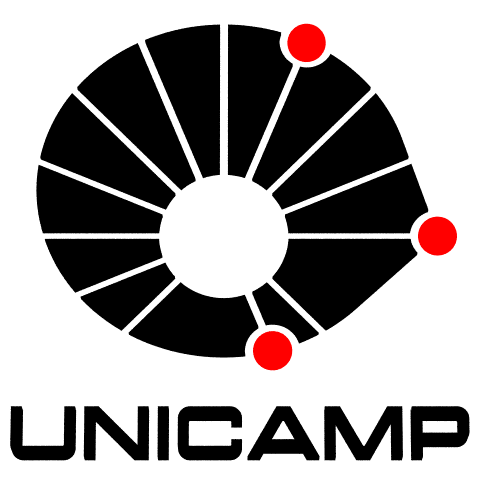
\includegraphics[height=0.07\textwidth]{Unicamp}}
        {Part-time Masters degree without being officially enrolled.
        %-------------------
        % set row color
        \newcommand{\rowgray}{\rowcolor[gray]{.95}}
        % set column separator
        \setlength{\tabcolsep}{3pt}
        %-------------------
        \begin{table}[H]
            \tiny
            \begin{center}
                \begin{tabular}{ |C{6.5mm}|m{6cm}|C{6mm}|m{2.6cm}|C{7.5mm}|C{9mm}| } 
                %              { |    subject    | cred |  prof  | semest | grade| } 
                    %=======================================
                    \hline
                    \rowcolor[gray]{0.75}
                    \multicolumn{2}{|c|}{Subject} & Credits & \multicolumn{1}{c|}{Professor(s)} & Semester & Grade \\
                    %=======================================
                    \hline
                    %-------------------
                    IA353A                                      &
                    Redes Neurais                               & 
                    4                                           & 
                    Fernando José Von Zuben                     &
                    1s2020                                      &
                    in progress                                 \\
                    %=======================================
                    \hline
                    \rowgray
                    & Tópicos Em Engenharia de Computação VII &&&&\\ 
                    %-------------------
                    \rowgray
                    \multirow{-2}{*}{IA376E}                    &
                    \hspace{1mm} $\hookrightarrow$ Redes Neurais Profundas Para Processamento de Linguagem Natural &
                    \multirow{-2}{*}{4}                         & 
                    \multirow{-2}{*}{Roberto de Alencar Lotufo} & 
                    \multirow{-2}{*}{1s2020}                    & 
                    \multirow{-2}{*}{in progress}               \\
                    %=======================================
                    \hline
                    %-------------------
                    \multirow{2}{*}{IA006C}                     & 
                    Tópicos em Sistemas Inteligentes II         & 
                    \multirow{2}{*}{4}                          & 
                    Levy Boccato                                & 
                    \multirow{2}{*}{2s2019}                     & 
                    \multirow{2}{*}{A}                          \\
                    %-------------------
                    & \hspace{1mm} $\hookrightarrow$ Aprendizado de Máquina && Romis Ribeiro de Faissol Attux &&\\
                    %=======================================
                    \hline
                    \rowgray
                    & Tópicos em Engenharia de Computação V     &&
                    Eleri Cardozo                               &&\\ 
                    %-------------------
                    \rowgray
                    \multirow{-2}{*}{IA368N}                    &
                    \hspace{1mm} $\hookrightarrow$ Introdução à Robótica Móvel &
                    \multirow{-2}{*}{4}                         & 
                    Eric Rohmer                                 &
                    \multirow{-2}{*}{2s2017}                    & 
                    \multirow{-2}{*}{A}                         \\
                    %=======================================
                    \hline
                    %-------------------
                    IA750A                                      & 
                    Engenharia de Reabilitação                  & 
                    4                                           & 
                    Antonio Augusto Fasolo Quevedo              & 
                    2s2017                                      & 
                    A                                           \\
                    %=======================================
                    \hline
                    \rowgray
                    & Tópicos em Engenharia de Computação V     &&
                    Eleri Cardozo                               &&\\ 
                    %-------------------
                    \rowgray
                    \multirow{-2}{*}{IA368W}                    & 
                    \hspace{1mm} $\hookrightarrow$ Métodos Estocásticos Para Robótica Móvel &
                    \multirow{-2}{*}{4}                         &
                    Eric Rohmer                                 &
                    \multirow{-2}{*}{1s2017}                    & 
                    \multirow{-2}{*}{A}                         \\
                    %=======================================
                    \hline
                    %-------------------
                    \multirow{2}{*}{IE327P}                     & 
                    Tópicos Especiais em Microeletrônica III    & 
                    \multirow{2}{*}{4}                          & 
                    \multirow{2}{*}{Elnatan Chagas Ferreira}    & 
                    \multirow{2}{*}{1s2017}                     & 
                    \multirow{2}{*}{A}                          \\
                    %-------------------
                    & \hspace{1mm} $\hookrightarrow$ Sensores, Condicionamento e Aquisição de Dados &&&&\\
                    %=======================================
                    \hline
                    \multicolumn{6}{l}{ }\\
                    \multicolumn{6}{r}{*table information in Portuguese}
                    %=======================================
                \end{tabular}
            \end{center}
            %\caption{}
            %\label{tab:}
        \end{table}
        }
    \vspace{-8mm}

    %---------------------------------------
    \profiledivider
    %---------------------------------------
	\cvevent
        {Undergraduate}
        {University of Campinas}
        {Jan 2011 -- Dec 2016}
        {Campinas/SP}
        {\hspace{2mm}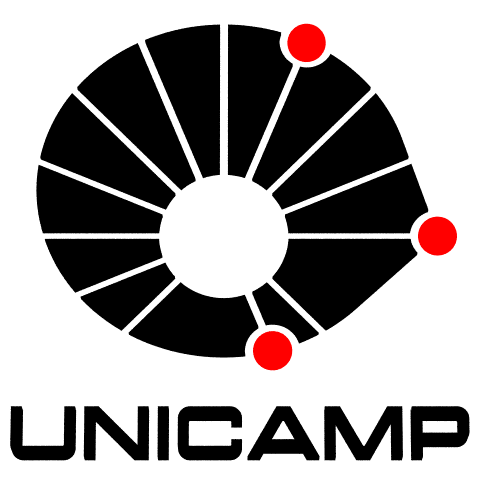
\includegraphics[height=0.07\textwidth]{Unicamp}}
        { 
        \vspace{-2mm}
        % set column separator
        \setlength{\tabcolsep}{3pt}
        \begin{table}[H]
            \tiny
            \begin{center}
                \begin{tabular}{ |C{6.5mm}|m{5.8cm}|C{6mm}|C{2.1cm}|C{17.5mm}|C{6mm}| }
                %              { |     subject     | cred |  prof  | semestr | grade| }
                    \hline
                    \rowcolor[gray]{0.75}
                    \multicolumn{2}{|c|}{Subject} & Credits & Professor & Semester & Grade \\
                    %=======================================
                    \hline
                    \multirow{2}{*}{EA999A}                     &
                    Tópicos em Egenharia de Computação          &
                    \multirow{2}{*}{4}                          &
                    \multirow{2}{*}{Roberto de Alencar Lotufo}  &
                    \multirow{2}{*}{Férias de Verão 2020}       &
                    \multirow{2}{*}{8.9}                        \\
                    %-------------------
                    & \hspace{1mm} $\hookrightarrow$ Curso Teórico-Prático de Redes Neurais Convolucionais &&&&\\
                    %=======================================
                    \hline
                    \multicolumn{6}{l}{ }\\
                    \multicolumn{6}{r}{*table information in Portuguese}
                    %=======================================
                 \end{tabular}
            \end{center}
            %\caption{}
            %\label{tab:}
        \end{table}
        }
    \vspace{-8mm}

    %---------------------------------------
    \profiledivider
    %---------------------------------------
    \cvevent
        {Undergraduate (Student Exchange Program)}
        {Queen Mary University of London}
        {Sep 2014 -- Aug 2015}
        {London}
        {\hspace{2mm}
\includegraphics[height=0.07\textwidth]{QMUL}}
        {Studies sponsored by the Brazilian government due to academic merit. Science without Borders (SwB) student exchange program.}

    %---------------------------------------
    \profiledivider
    %---------------------------------------
	\cvevent
        {Further Education}
        {Technical College of Campinas - UNICAMP}
        {Jan 2007 -- Jul 2010}
        {Campinas/SP}
        {\hspace{2mm}
\includegraphics[height=0.07\textwidth]{Cotuca}}
        {Selected to work as a Teaching Assistant of the technical course.}

%=======================================
\cvsection{Machine Learning Portfolio}
%=======================================
%-------------------
% change item symbols
\renewcommand{\labelitemi}{\textbullet}
\renewcommand{\labelitemii}{\textbullet}
\renewcommand{\labelitemiii}{\textbullet}
\renewcommand{\labelitemiv}{\textbullet}
%-------------------
% include images path
\graphicspath{{../figures/machine-learning-portfolio/}}
% GitHub icon
\newcommand{\github}[1]{\href{#1}{\faGithub}}
% Google Colab icon
\newcommand{\colab}[1]{\href{#1}{\includegraphics[height=1em]{colab}}}
%-------------------
%\begin{multicols}{2}
%\begin{vwcol}[widths={0.45,0.55}, sep=.8cm, justify=flush,rule=0pt,indent=1em]
\begin{minipage}[t]{0.45\linewidth}

\small
\textbf{\color{sectioncolor}Jupyter notebooks:}\\\\
\scriptsize
%---------------------------------------
\textbf{\underline{Computer Vision:}}
%---------------------------------------
\begin{itemize}[leftmargin=*,labelindent=3mm,labelsep=1mm]
    %---------------------------------------
    \item MNIST: Linear Classifier
        \hfill
        \github{https://github.com/ito-rafael/machine-learning/blob/master/notebooks/computer\%20vision/MNIST\%20-\%20Linear.ipynb}
        \hspace{0.1mm}
        \colab{https://colab.research.google.com/drive/1QTgLwLK3BEfQV0fi_HasQsL1Zm-6l4A4?usp=sharing}
    %---------------------------------------
    \item MNIST: Extreme Learning Machine (ELM)
        \hfill
        \github{https://github.com/ito-rafael/machine-learning/blob/master/notebooks/computer\%20vision/MNIST\%20-\%20ELM.ipynb}
        \hspace{0.1mm}
        \colab{https://colab.research.google.com/drive/1FUbVaGFz9UmNx9NP45wHZC0Of7WMz75r?usp=sharing}
    %---------------------------------------
    \item MNIST: Multilayer Perceptron (MLP)
        \hfill
        \github{https://github.com/ito-rafael/machine-learning/blob/master/notebooks/computer\%20vision/MNIST\%20-\%20MLP.ipynb}
        \hspace{0.1mm}
        \colab{https://colab.research.google.com/drive/1OKWU4uYmgj7YWWC8o2UKolOPtqimSBfK?usp=sharing}
    %---------------------------------------
    \item MNIST: ConvNet (CNN)
        \hfill
        \github{https://github.com/ito-rafael/machine-learning/blob/master/notebooks/computer\%20vision/MNIST\%20-\%20ConvNet.ipynb}
        \hspace{0.1mm}
        \colab{https://colab.research.google.com/drive/1Ne6y2G_rsH4bYoItFveRA29N0NZ9ZZL_?usp=sharing}
    %---------------------------------------
    \item Transfer Learning: Cats and Dogs
        \hfill
        \github{https://github.com/ito-rafael/machine-learning/blob/master/notebooks/computer\%20vision/Transfer\%20Learning\%20-\%20Cats\%20\%26\%20Dogs.ipynb}
        \hspace{0.1mm}
        \colab{https://colab.research.google.com/drive/1okJH91odJWQXn5pScQfVyjkAYTvH06Sk}
    %---------------------------------------
    \item Transfer Learning (last layer): Fruits360
        \hfill
        \github{https://github.com/ito-rafael/machine-learning/blob/master/notebooks/computer\%20vision/Transfer\%20Learning\%20-\%20Fruits360\%20(only\%20last\%20layer).ipynb}
        \hspace{0.1mm}
        \colab{https://colab.research.google.com/drive/18d_M9U0uxQ0lAOqoiHA18ekjQq4xNX4D}
    %---------------------------------------
    \item Transfer Learning (fine tuning): Fruits360
        \hfill
        \github{https://github.com/ito-rafael/machine-learning/blob/master/notebooks/computer\%20vision/Transfer\%20Learning\%20-\%20Fruits360\%20(fine-tunning).ipynb}
        \hspace{0.1mm}
        \colab{https://colab.research.google.com/drive/1R9xNZk7E1C-_5x_AW_r2PA5NDBrNqKEb}
    %---------------------------------------
\end{itemize}
\vspace{2mm}

%---------------------------------------
\textbf{\underline{Natural Language Processing (NLP):}}
%---------------------------------------
\begin{itemize}[leftmargin=*,labelindent=3mm,labelsep=1mm]
    %---------------------------------------
    \item Language Model
        \hfill
        \github{https://github.com/ito-rafael/IA376E-NLP_DeepLearning-1s2020/blob/master/Aula\%203/Language_Model_(Rafael_Ito).ipynb}
        \hspace{0.1mm}
        \colab{https://colab.research.google.com/drive/1bN7PZKTg5tNFbshVDpeDs2SyO0ry7t-g}
    %---------------------------------------
    \item Sentiment Analysis (IMDb dataset) using:
    \begin{itemize}[leftmargin=*,labelindent=2mm,labelsep=1mm]
        %-------------------
        \item Bag-of-Words
            \hfill
            \github{https://github.com/ito-rafael/IA376E-NLP_DeepLearning-1s2020/blob/master/Aula\%202/IMDb_Sentiment_analysis_(Rafael_Ito).ipynb}
            \hspace{0.1mm}
            \colab{https://colab.research.google.com/drive/1CTPhLShW60HhVE0zzQFTq45jRiEKPKcR}
        %-------------------
        \item TF-IDF
            \hfill
            \github{https://github.com/ito-rafael/IA376E-NLP_DeepLearning-1s2020/blob/master/Aula\%204/IMDb_Sentiment_analysis_with_(Rafael_Ito).ipynb}
            \hspace{0.1mm}
            \colab{https://colab.research.google.com/drive/1ynG17D67-hi78xPcEkHzxalsaMmut9z6}
        %-------------------
        \item Simplified Self-Attention
            \hfill
            \github{https://github.com/ito-rafael/IA376E-NLP_DeepLearning-1s2020/blob/master/Aula\%205/IMDb_Sentiment_analysis_(Self_Attention_simple)_(Rafael_Ito).ipynb}
            \hspace{0.1mm}
            \colab{https://colab.research.google.com/drive/1DZKqRb-wW8waV2z27KQFKQHD73p5QxIQ}
        %-------------------
        \item Transformer (Encoder only)
            \hfill
            \github{https://github.com/ito-rafael/IA376E-NLP_DeepLearning-1s2020/blob/master/Aula\%206/IMDb_Sentiment_analysis_(Self_Attention_complete)_(Rafael_Ito).ipynb}
            \hspace{0.1mm}
            \colab{https://colab.research.google.com/drive/1G1qezkPK8HNyX3JuaqthZYgLnvz_fDvY}
        %-------------------
        \item BERT
            \hfill
            \github{https://github.com/ito-rafael/IA376E-NLP_DeepLearning-1s2020/blob/master/Aula\%208/Aula_8_BERT_(Rafael_Ito).ipynb}
            \hspace{0.1mm}
            \colab{https://colab.research.google.com/drive/1N6cw_YLv9bBXqF82b4pM_KJ3ms_-4o5z?authuser=1}
        %-------------------
    \end{itemize}
    %---------------------------------------
    \item T5 English to Portuguese Translator
            \hfill
            \github{https://github.com/ito-rafael/IA376E-NLP_DeepLearning-1s2020/blob/master/Aula\%209/Aula_9_T5_(English_Portuguese_translation)_(Rafael_Ito).ipynb}
            \hspace{0.1mm}
            \colab{https://colab.research.google.com/drive/192AWnbDwBnVX0uKiDF7dRfYH-1MxAd15}
\end{itemize}
\vspace{2mm}

%---------------------------------------
\textbf{\underline{Video Processing:}}
%---------------------------------------
\begin{itemize}[leftmargin=*,labelindent=3mm,labelsep=1mm]
    %---------------------------------------
    \item YOLO
        \hfill
        ...in progress
%        \github{https://github.com/ito-rafael/IA376E-NLP_DeepLearning-1s2020/blob/master/Aula\%203/Language_Model_(Rafael_Ito).ipynb}
%        \hspace{0.1mm}
%        \colab{https://colab.research.google.com/drive/1bN7PZKTg5tNFbshVDpeDs2SyO0ry7t-g}
    %---------------------------------------
    \item MobileNets
        \hfill
        ...in progress
%        \github{https://github.com/ito-rafael/IA376E-NLP_DeepLearning-1s2020/blob/master/Aula\%203/Language_Model_(Rafael_Ito).ipynb}
%        \hspace{0.1mm}
%        \colab{https://colab.research.google.com/drive/1bN7PZKTg5tNFbshVDpeDs2SyO0ry7t-g}
    %---------------------------------------
\end{itemize}
%---------------------------------------

\end{minipage}
\hspace{1mm}
%=======================================
\begin{minipage}[t]{0.53\linewidth}
\small
\textbf{\color{sectioncolor}One-page papers summary:}
\vspace{1.0mm}\\
\scriptsize
*available only in Portuguese

%-------------------
% Google Drive icon
\newcommand{\drive}[1]{\href{#1}{\includegraphics[height=1em]{drive}}}
% PDF icon
\newcommand{\pdf}[1]{\href{#1}{\hspace{1mm}\includegraphics[height=1em]{pdf}\\}}
%-------------------
\begin{itemize}[leftmargin=*,labelindent=3mm,labelsep=1mm]
    %---------------------------------------
    \item "A Neural Probabilistic Language Model", 2003
    %---------------------------------------
%        \hfill
        \pdf{http://www.jmlr.org/papers/volume3/bengio03a/bengio03a.pdf}
        \hfill
        \hspace{2mm} $\hookrightarrow$ summary: 
            \github{https://github.com/ito-rafael/machine-learning/blob/master/one-page\%20papers\%20summary/2003\%20-\%20\%5BLanguage\%20Model\%5D\%20A\%20Neural\%20Probabilistic\%20Language\%20Model\%20\%5BYoshua\%20Bengio\%20-\%20Universit\%C3\%A9\%20de\%20Montr\%C3\%A9al\%5D.pdf}
            \hspace{0.1mm}
            \drive{https://docs.google.com/document/d/1MBboy05JIT-TyNyTxl-ppMgO-4PvaaaZrnW-M1L-0yI/edit?usp=sharing}
    %---------------------------------------
    \item "A Unified Architecture for Natural Language Processing: Deep Neural Networks with Multitask Learning", 2008
    %---------------------------------------
%        \hfill
        \pdf{https://ronan.collobert.com/pub/matos/2008_nlp_icml.pdf}
        \hfill
        \hspace{2mm} $\hookrightarrow$ summary: 
            \github{https://github.com/ito-rafael/machine-learning/blob/master/one-page\%20papers\%20summary/2008\%20-\%20\%5BMultitask\%20NLP\%5D\%20A\%20Unified\%20Architecture\%20for\%20Natural\%20Language\%20Processing:\%20Deep\%20Neural\%20Networks\%20with\%20Multitask\%20Learning\%20\%5BRonan\%20Collobert\%2C\%20Jason\%20Weston\%5D.pdf} 
            \hspace{0.1mm}
        \drive{https://docs.google.com/document/d/1jd6sd-SxfUYHUdh8hbLCDcR_PZ11d51tiEEHWcL3-zE/edit?usp=sharing} 
    %---------------------------------------
    \item "Efficient Estimation of Word Representations in Vector Space", 2013
    %---------------------------------------
%        \hfill
        \pdf{https://arxiv.org/pdf/1301.3781.pdf}
        \hfill
        \hspace{2mm} $\hookrightarrow$ summary: 
            \github{https://github.com/ito-rafael/machine-learning/blob/master/one-page\%20papers\%20summary/2013\%20-\%20\%5Bword2vec\%5D\%20Efficient\%20Estimation\%20of\%20Word\%20Representations\%20in\%20Vector\%20Space\%20\%5BGoogle\%20Inc\%5D.pdf} 
            \hspace{0.1mm}
            \drive{https://docs.google.com/document/d/11MRzz4_oK4KjUcnqLXI2B7Z2WDYRz7PtxctMZcjm2GA/edit?usp=sharing} 
    %---------------------------------------
    \item "Deep Learning", 2015
    %---------------------------------------
 %       \hfill
        \pdf{https://s3.us-east-2.amazonaws.com/hkg-website-assets/static/pages/files/DeepLearning.pdf}
        \hfill
        \hspace{2mm} $\hookrightarrow$ summary: 
            \github{https://github.com/ito-rafael/machine-learning/blob/master/one-page\%20papers\%20summary/2015\%20-\%20\%5BDeep\%20Learning\%5D\%20Deep\%20Learning\%20\%5BYann\%20LeCun\%2C\%20Yoshua\%20Bengio\%2C\%20Geoffrey\%20Hinton\%5D.pdf}
            \hspace{0.1mm}
            \drive{https://docs.google.com/document/d/1RW47cxVSiQoWAZ74jlFNnT6s5Q_6Ey7ua_uIBcmNBeg/edit?usp=sharing}
    %---------------------------------------
    \item "Effective Approaches to Attention-based Neural Machine Translation", 2015
    %---------------------------------------
%        \hfill
        \pdf{https://arxiv.org/pdf/1508.04025.pdf}
        \hfill
        \hspace{2mm} $\hookrightarrow$ summary: 
            \github{https://github.com/ito-rafael/machine-learning/blob/master/one-page\%20papers\%20summary/2015\%20-\%20\%5BAttention\%20NMT\%5D\%20Effective\%20Approaches\%20to\%20Attention-based\%20Neural\%20Machine\%20Translation\%20\%5BStanford\%5D.pdf} 
            \hspace{0.1mm}
            \drive{https://docs.google.com/document/d/13iF8bPHbeW97mOck_Ncqxtt_U4vkHXtaPbkqE-sPcww/edit?usp=sharing} 
    %---------------------------------------
    \item "Attention Is All You Need", 2017
    %---------------------------------------
%        \hfill
        \pdf{https://arxiv.org/pdf/1706.03762.pdf}
        \hfill
        \hspace{2mm} $\hookrightarrow$ summary: 
            \github{https://github.com/ito-rafael/machine-learning/blob/master/one-page\%20papers\%20summary/2017\%20-\%20\%5BTransformer\%5D\%20Attention\%20Is\%20All\%20You\%20Need\%20\%5BGoogle\%20Brain\%5D\%20(Vaswani\%20et\%20al.\%2C\%202017).pdf} 
            \hspace{0.1mm}
            \drive{https://docs.google.com/document/d/1pCnipY7b_Qcs0w1HAw8W9jDGRrzmH1KixT9Rlg8Mu0E/edit?usp=sharing} 
    %---------------------------------------
    \item "BERT: Pre-training of Deep Bidirectional Transformers for Language Understanding", 2019
    %---------------------------------------
%        \hfill
        \pdf{https://arxiv.org/pdf/1810.04805.pdf}
        \hfill
        \hspace{2mm} $\hookrightarrow$ summary: 
            \github{https://github.com/ito-rafael/machine-learning/blob/master/one-page\%20papers\%20summary/2019\%20-\%20\%5BBERT\%5D\%20BERT:\%20Pre-training\%20of\%20Deep\%20Bidirectional\%20Transformers\%20for\%20Language\%20Understanding\%20\%5BGoogle\%20AI\%20Language\%5D\%20(Devlin\%20et\%20al.\%2C\%202019).pdf} 
            \hspace{0.1mm}
            \drive{https://docs.google.com/document/d/1Yrd7j6UAQkS0ZHbjl-893eqiQuCVXFj1b4tOv2QHb1w/edit?usp=sharing} 
    %---------------------------------------
    \item "Exploring the Limits of Transfer Learning with a Unified Text-to-Text Transformer", 2019
    %---------------------------------------
%        \hfill
        \pdf{https://arxiv.org/pdf/1910.10683.pdf}
        \hfill
        \hspace{2mm} $\hookrightarrow$ summary: 
            \github{https://github.com/ito-rafael/machine-learning/blob/master/one-page\%20papers\%20summary/2019\%20-\%20\%5BT5\%5D\%20Exploring\%20the\%20Limits\%20of\%20Transfer\%20Learning\%20with\%20a\%20Unified\%20Text-to-Text\%20Transformer\%20\%5BGoogle\%5D.pdf} 
            \hspace{0.1mm}
            \drive{https://docs.google.com/document/d/13HLEYCKsRb_EJRauQyZpAOuXUhTC4GrDlFDhW5l-A-o/edit?usp=sharing} 
    %---------------------------------------
    \item "The Curious Case of Neural Text Degeneration", 2019
    %---------------------------------------
%        \hfill
        \pdf{https://arxiv.org/pdf/1904.09751.pdf}
        \hfill
        \hspace{2mm} $\hookrightarrow$ summary: 
            \github{https://github.com/ito-rafael/machine-learning/blob/master/one-page\%20papers\%20summary/2019\%20-\%20\%5BNucleus\%20Sampling\%5D\%20The\%20Curious\%20Case\%20of\%20Neural\%20Text\%20Degeneration\%20\%5BAllen\%20Institute\%20for\%20Artificial\%20Intelligence\%5D.pdf} 
            \hspace{0.1mm}
            \drive{https://docs.google.com/document/d/1IcBG9UQJNIfzteAGzPU7q-_wfBZnGPQ4H5GUwI-Q7EQ/edit?usp=sharing} 
    %---------------------------------------

\end{itemize}

\end{minipage}
%\end{multicols}
%\end{vwcol}

%%=======================================
%\cvsection{Awards}
%%=======================================
%\begin{cvtable}
%	\cvitem{2010 -- now}{Panda of the Year}{Panda World Forum}{}
%	\cvitem{2005 -- now}{Face of World Wide Fund for Nature}{WWF}{}
%	\cvitem{2000}{Winner of Bamboo Sprouts Eating Contest}{Bamboo Society}{}
%\end{cvtable}
%
%
%%=======================================
%\cvsection{Extra-Curricular Activities}
%%=======================================
%\begin{cvtable}
%	\cvitemshort{Relaxing}{Master the fine art of relaxing everywhere}
%	\cvitemshort{Music}{Playing the bamboo flute in the 1st Panda Orchestra}
%	\cvitemshort{Education}{Teaching young pandas to be more panda-like}
%\end{cvtable}

%===============================================================================
%                         TABLE ENTRIES 2nd PAGE
%===============================================================================
\newpage
\makebacksidebar

%=======================================
\cvsection{Working Experience}
%=======================================
% change arraystretch (distance between items):
%\begin{cvtable}[<arraystretch>=1]
%\begin{cvtable}[1.5]
\graphicspath{{../figures/work/}}
\newcolumntype{L}{>{\centering\arraybackslash}m{5.5cm}}
%	%\cvitem
    \cvevent
        {Technological Development Analyst}
        {CNPEM/LNLS}
        {Jan 2016 -- current}
        {Campinas/SP}
        {\hspace{2mm}
\includegraphics[height=0.07\textwidth]{CNPEM}}
        {Blah}
    %---------------------------------------
    \\\profiledivider
    %---------------------------------------
	%\cvitem{Jan 2016 Jul 2016}{Teaching Assistant}{University of Campinas}{bla alkdjasjd asdjasd asiod asoidj asoid jasdj asoidj as djaskldjaslkd jalsdjlasjda daskl djalskdlajs ldasj dlkasj daskldj alsjdasld lasdasd aslj dlasdj asl djlas ldajl dasjd asl dlasjd\medskip}
	%\cvitem
    \cvevent
        {Teaching Assistant}
        {University of Campinas}
        {Jan 2016 -- Jul 2016}
        {Campinas/SP}
        {\hspace{2mm}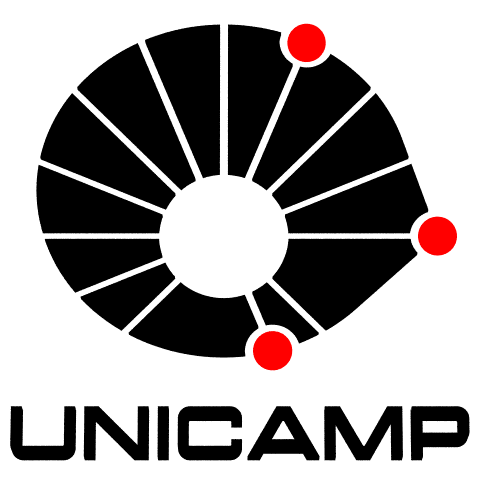
\includegraphics[height=0.07\textwidth]{Unicamp}}
        {\blindtext}
    %---------------------------------------
    \\\profiledivider
    %---------------------------------------
	%\cvitem
    \cvevent
        {Scientific Research}
        {Queen Mary University of London}
        {Jun 2015 -- Sep 2015}
        {London}
        {\hspace{2mm}
\includegraphics[height=0.07\textwidth]{QMUL}}
        {blabljdbjsdl bksdjblsdblds bjsd bkljsd blksjd blksdj blsd jblsd blksdjb lksdj blkds jblskd bjsdbjksdl bjlsdjblsd jblsdb sdlk bjlds jbsdkl bdsjl bkldsj blsd lbj s dblsdb sd kbj sdlkbjdskl bjdskl jbldsj b}
    %---------------------------------------
    \\\profiledivider
    %---------------------------------------
	%\cvitem{Jan 2010 Jun 2010}{Electronics intern}{CPqD - Telecommunications Research and Development Centre}{bla\medskip}
	%\cvitem
    \cvevent
        {Electronics intern}
        {CPqD - Telecommunications Research and Development Centre}
        {Jan 2010 -- Jun 2010}
        {Campinas/SP}
        {\hspace{2mm}
\includegraphics[height=0.07\textwidth]{CPqD}}
        {bla}
    %---------------------------------------
    \\\profiledivider
    %---------------------------------------
    %\cvitem
    \cvevent
        {Teaching Assistant}
        {Technical College of Campinas}
        {Jan 2009 -- Dec 2009}
        {Campinas/SP}
        {\hspace{2mm}
\includegraphics[height=0.07\textwidth]{Cotuca}}
        {bla}

%=======================================
\cvsection{Publications}
%=======================================
\begin{cvtable}
	\cvpubitem
        %http://icalepcs2019.vrws.de/papers/wempr003.pdf
        {Exploring Embedded Systems' Dedicated Cores for Real-Time Applications}
        {P. H. Nallin, G. R. S. Franco, R. C. Ito, and A. R. D. Rodrigues}
		{17th Int. Conf. on Accelerator and Large Experimental Physics Control Systems (ICALEPCS'19)}
        {October 2019}
        {New York, USA}
    %---------------------------------------
	\cvpubitem
        %http://icalepcs2019.vrws.de/papers/mopha031.pdf
        {Software and Hardware Design for Controls Infrastructure at Sirius Light Source}
        {G. R. S. Franco et al.}
        {17th Int. Conf. on Accelerator and Large Experimental Physics Control Systems (ICALEPCS'19)}
        {October 2019}
        {New York, USA}
\end{cvtable}
%=======================================

%\cvsection{section}
%\cvsubsection{Subsection}
%\begin{cvtable}
%	\cvitem{<dates>}{<cv-item title>}{<location>}{<optional: description>}
%\end{cvtable}
%
%\cvsection{cvitem}
%\cvsubsection{Multi-line with longer description}
%\begin{cvtable}
%	\cvitem{date}{Description}{location}{Some longer and more detailed
%		description, that takes two lines of space instead of only one.}
%	\cvitem{date}{Description}{location}{Some longer and more detailed
%		description, that takes two lines of space instead of only one.}
%	\cvitem{date}{Description}{location}{Some longer and more detailed
%		description, that takes two lines of space instead of only one.}
%\end{cvtable}
%
%\cvsubsection{One-line without description}
%\begin{cvtable}
%	\cvitem{Award}{One-line description}{Sponsor}{}
%	\cvitem{Award}{One-line description}{Sponsor}{}
%	\cvitem{Award}{One-line description}{Sponsor}{}
%\end{cvtable}
%
%\cvsection{cvitemshort}
%\cvsubsection{One-line}
%\begin{cvtable}
%	\cvitemshort{Key}{Some further description}
%	\cvitemshort{Key}{Some further description}
%	\cvitemshort{Key}{Some further description}
%\end{cvtable}
%
%\cvsubsection{Multi-line with longer description}
%\begin{cvtable}
%	\cvitemshort{Key}{Some further description. Can fill even more than
%		only one single line while still keeping the correct indendation level.}
%	\cvitemshort{Key}{Some further description. Can fill even more than
%		only one single line while still keeping the correct indendation level.}
%	\cvitemshort{Key}{Some further description. Can fill even more than
%		only one single line while still keeping the correct indendation level.}
%\end{cvtable}
%
%\cvsection{cvpubitem}
%\begin{cvtable}
%	\cvpubitem{Publication title}{Authors}{Journal}{Year}
%	\cvpubitem{Publication title}{Authors}{Journal}{Year}
%	\cvpubitem{Publication title that is spanning over multiple lines and still
%		does not look too bad}{Authors}{Journal}{Year}
%\end{cvtable}

\cvsignature

\end{document}
